\def\difficulty{2}

\sujet{Shape Diagrams}
\index{Characterization}

%\vspace*{-8pt}

\begin{note}The objective is to study some shape diagrams and the possibility to define properties that may be useful in order to distinguish the different objects.\end{note}

Shape diagrams are representations of single shapes (connected compact sets, see \cite{Rivollier2010a,Rivollier2010b,Rivollier2010c}) as points in the 2-D unit square plane. They are based on inequalities between 6 geometrical measurements: area $A$, perimeter $P$, radius of the inscribed circle $r$, radius of the circumscribed circle $R$, minimum Feret diameter $\omega$ and maximum Feret diameter $d$. In this way, the morphometrical functionals used in the different shape diagrams are normalized ratios of such geometrical functionals. The following table shows the morphometrical functionals for non-convex sets:

%\begin{table}[!htbp]
%\caption{Inequalities between geometrical functionals and the corresponding morphometrical functionals, not restricted to compact convex sets.} \label{tab:MorphomFuncs}
\begin{table}[htbp]
\centering
    \begin{tabular}{|c@{\hspace{0.4cm}}|c@{\hspace{0.4cm}}|c@{\hspace{0.4cm}}|}
        \hline
        %\textbf{Geometrical functionals} & \textbf{Inequalities} & \textbf{Morphological functionals} & \textbf{extremal sets} \\
        \begin{tabular}{@{}c@{}}{Geometrical} \\ {functionals}\end{tabular} & {Inequalities} & \begin{tabular}{@{}c@{}}{Morphological} \\ {functionals}\end{tabular} \\
        \hline
        $r$, $R$ & $r \leq R$ & $r / R$  \\
        $\omega$, $R$ & $\omega \leq 2R$ & $\omega / 2R$  \\
        $A$, $R$ & $A \leq \pi R^2$ & $A / \pi R^2$  \\
        $d$, $R$ & $d \leq 2R$ & $d / 2R$  \\
        \hline
        $r$, $d$ & $2r \leq d$ & $2r / d$  \\
        $\omega$, $d$ & $\omega \leq d$ & $\omega / d$  \\
        $A$, $d$ & $4A \leq \pi d^2$ & $4A / \pi d^2$  \\
        $R$, $d$ & $\sqrt{3}R \leq d$ & $\sqrt{3}R / d$  \\
        \hline
        $r$, $P$ & $2\pi r \leq P$ & $2\pi r / P$  \\
        $\omega$, $P$ & $\pi \omega \leq P$ & $\pi \omega / P$  \\
        $A$, $P$ & $4\pi A \leq P^2$ & $4\pi A / P^2$  \\
        $d$, $P$ & $2d \leq P$ & $2d / P$  \\
        $R$, $P$ & $4R \leq P$ & $4R / P$  \\
        \hline
        $r$, $A$ & $\pi r^2 \leq A$ & $\pi r^2 / A$  \\
        \hline
        $r$, $\omega$ & $2r \leq \omega$ & $2r / \omega$  \\
        \hline
    \end{tabular}
 \caption{Morphometrical functionals.}
 \label{tab:shape_diagram:enonce:functionals}
\end{table}

\vspace*{-10pt}

\begin{figure}[H]
\centering\caption[Kimia image database.]{The different processes will be applied on images from the Kimia database \cite{KimiaDB,Sharvit1998}.}%
\subfloat[Apple.]{
\includegraphics[height=.28\linewidth]{apple-3.png}}\hfill
\subfloat[Bone.]{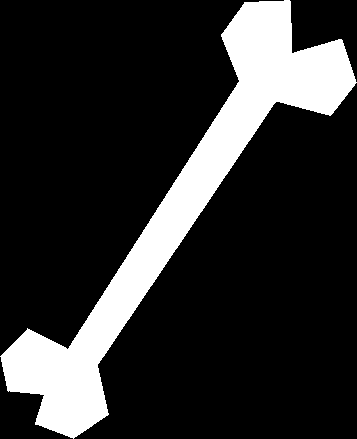
\includegraphics[height=.28\linewidth]{Bone-3.png}}\hfill
\subfloat[Camel.]{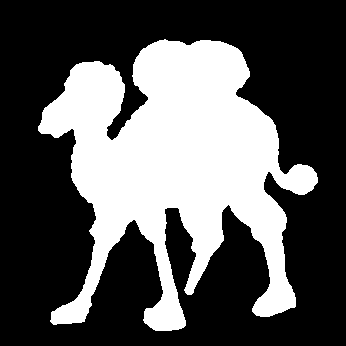
\includegraphics[height=.28\linewidth]{camel-3.png}}%
\vspace*{-8pt}
% http://vision.lems.brown.edu/content/available-software-and-databases
\end{figure}


%\newpage
\section{Geometrical functionals}
\vspace*{-10pt}
\begin{qbox}
Code functions in order to evaluate the different parameters:\vspace*{-8pt}
  \begin{itemize}
  \item the area, Crofton perimeter and Feret diameters have been already presented in \iflabelexists{tutorial:integral_geometry:enonce}{tutorial \ref{tutorial:integral_geometry:enonce}}{the tutorial about integral geometry};
	\item \textls[-25]{the radius of the inscribed circle can be defined from the ultimate erosion of a set.}  
	%\item the algorithm for computing the circumscribed circle is not simple and out of the scope of this tutorial. Some functions are provided for convenience.
 \end{itemize}
\end{qbox}

\vspace*{-8pt}

\begin{mcomment}
\begin{mremark}
The function \minline{bwdist} computes the distance map of a binary image.
\end{mremark}
\end{mcomment}

\begin{pcomment}
\begin{premark}
The function \pinline{scipy.ndimage.morphology.distance_transform_cdt} computes the distance map of a binary image (chamfer distance transform).
\end{premark}
\end{pcomment}

\vspace*{-18pt}
\section{Morphometrical functionals}\vspace*{-10pt}
\begin{qbox} \textls[-10]{Code and evaluate some of the morphometrical functionals listed in the table \ref{tab:shape_diagram:enonce:functionals}. Note that each of them has a physical meaning, e.g. $\frac{4\pi A}{P^2}$ (circularity), $\frac{4A}{\pi d^2}$ (roundness), $2\omega/P$ (thinness).}
\end{qbox}

\vspace*{-10pt}

\section{Shape diagrams}\vspace*{-10pt}
\begin{qbox}
\begin{itemize}
	\item Visualize the different shape diagrams for all the images (from the Kimia database) within the three classes 'apple', 'bone' and 'camel'. The Fig.\ref{fig:enonce:shape_diagram:diag3} illustrates the result for the shape diagram $(x=2r/d, y=P/\pi d)$.

	\item \textls[-30]{Which shape diagram is the most appropriate for the discrimination of such objects?}
\end{itemize}
\end{qbox}

\vspace*{-10pt}%\enlargethispage{2pt}

\begin{figure}[H]
  \centering\caption{Example of a shape diagram.}%
   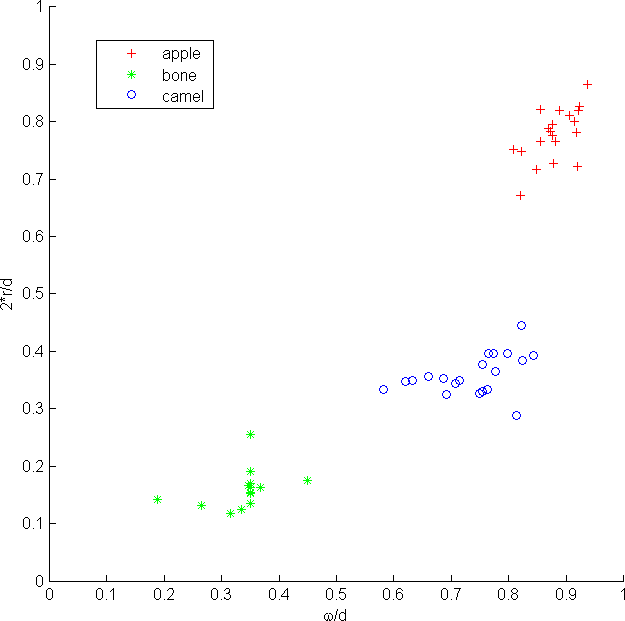
\includegraphics[width=5cm]{shape_diagramT}%
   \label{fig:enonce:shape_diagram:diag3}%
  \end{figure}\vspace*{-20pt}
\section{Shape classification}\vspace*{-10pt}
\index{Segmentation!K-means}
\begin{qbox}
\begin{itemize}
	\item Use a K-means clustering method  for automatic classification of such shapes.
	\item \textls[-10]{Propose a method to quantify the classification accuracy for each shape diagram.}
\end{itemize}
\end{qbox}
